\section{Auswertung}
\label{sec:Auswertung}

\subsection{Messung der Magnetfelder verschiedener Spulen}

\subsubsection{Lange Spule}
  \begin{table}
    \centering
    \caption{Messdaten der langen Spule.}
    \label{tab:lang}
    \sisetup{table-format=1.3}
    \begin{tabular}{S[table-format=2] S}
    \toprule
    {$x \:/\: \si{\cm}$} & {$B \:/\: \si{\milli\tesla}$}\\
    \midrule
          4 & 0.079\\
          3 & 0.139\\
          2 & 0.258\\
          1 & 0.506\\
          0 & 0.971\\
          -1 & 1.524\\
          -2 & 1.888\\
          -3 & 2.077\\
          -4 & 2.165\\
          -5 & 2.213\\
        \bottomrule
      \end{tabular}
    \end{table}

\begin{figure}
  \centering
  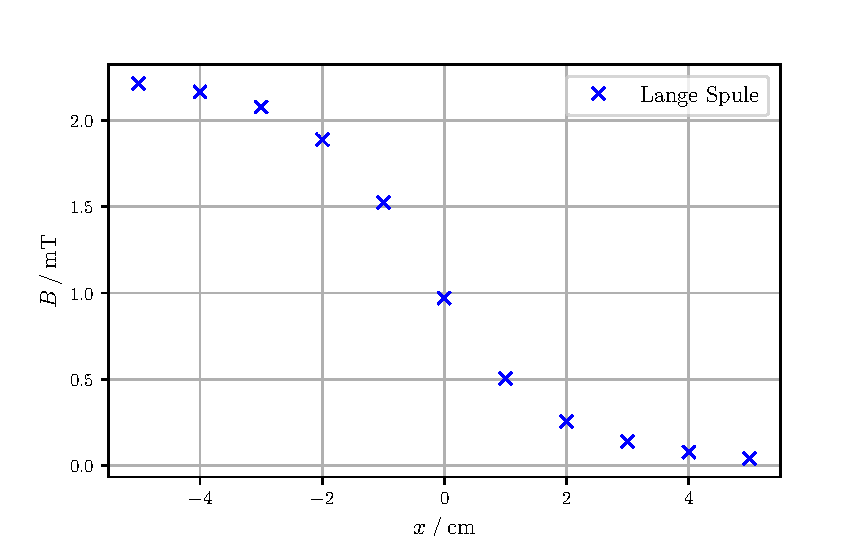
\includegraphics[width=\textwidth]{build/lange_Spule.pdf}
  \caption{Messdaten der langen Spule.}\label{fig:lang}
\end{figure}



\subsubsection{Kurze Spule}
  \begin{table}
    \centering
    \caption{Messdaten der kurzen Spule.}
    \label{tab:kurz}
    \sisetup{table-format=1.3}
    \begin{tabular}{S[table-format=2] S}
    \toprule
    {$x \:/\: \si{\cm}$} & {$B \:/\: \si{\milli\tesla}$}\\
    \midrule
          5 & 0.048\\
          4 & 0.076\\
          3 & 0.131\\
          2 & 0.247\\
          1 & 0.470\\
          0 & 0.886\\
          -1 & 1.405\\
          -2 & 1.770\\
          -3 & 1.882\\
          -4 & 1.812\\
          -5 & 1.530\\
          \bottomrule
  \end{tabular}
\end{table}

\begin{figure}
  \centering
  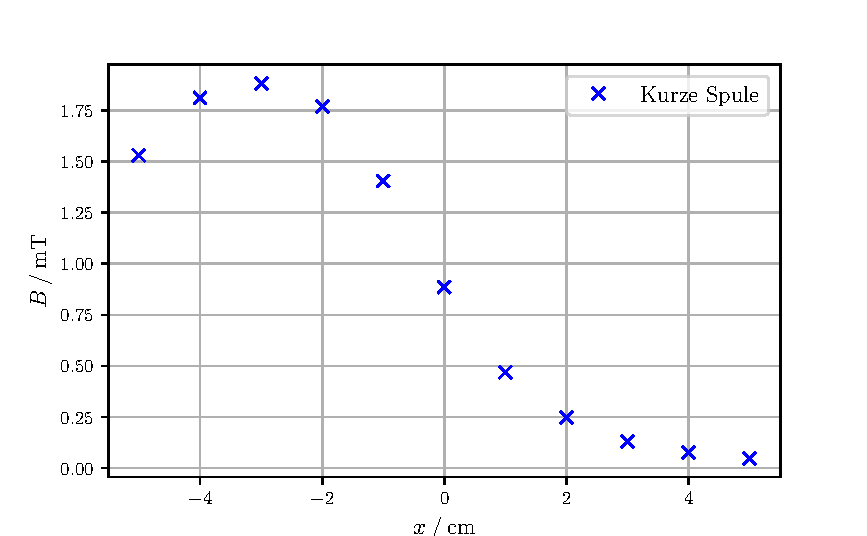
\includegraphics[width=\textwidth]{build/kurze_Spule.pdf}
  \caption{Messdaten der kurzen Spule.}\label{fig:kurz}
\end{figure}


\subsubsection{Dicke Spule}
  \begin{table}
    \centering
    \caption{Messdaten der dicken Spule.}
    \label{tab:dick}
    \sisetup{table-format=1.3}
    \begin{tabular}{S[table-format=2] S}
    \toprule
    {$x \:/\: \si{\cm}$} & {$B \:/\: \si{\milli\tesla}$}\\
    \midrule
        5 & 1.56\\
        4 & 2.00\\
        3 & 2.58\\
        2 & 3.31\\
        1 & 4.22\\
        0 & 5.18\\
        -1 & 6.13\\
        -2 & 7.01\\
        -3 & 7.64\\
        -4 & 7.99\\
        -5 & 8.03\\
        \bottomrule
      \end{tabular}
    \end{table}


\begin{figure}
  \centering
  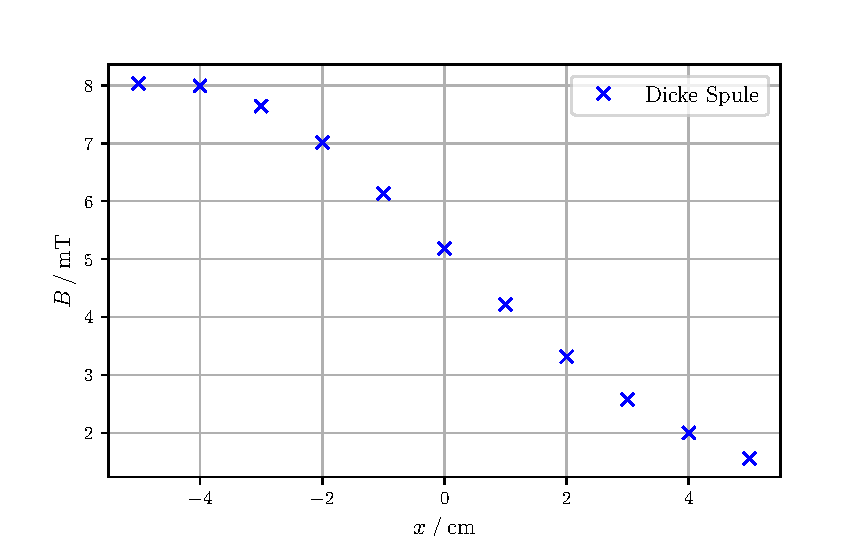
\includegraphics[width=\textwidth]{build/dicke_Spule.pdf}
  \caption{Messdaten der dicken Spule.}\label{fig:dick}
\end{figure}


\subsection{Helmholtz-Spulen-Paar}
  \begin{table}
    \centering
    \caption{Messdaten des Helmholtz-Spulen-Paares.}
    \label{tab:helmholtz}
    \begin{tabular}{S[table-format=2.1] S[table-format=1.2] S[table-format=2.1] S[table-format=1.3] S[table-format=2.1] S[table-format=1.3]}
    \toprule
    \multicolumn{2}{l}{Spulenabstand: $12.5 \si{\cm}$} & \multicolumn{2}{l}{Spulenabstand: $6.25 \si{\cm}$} & \multicolumn{2}{l}{Spulenabstand: $18.75 \si{\cm}$}\\
      \cmidrule(lr){1-2}\cmidrule(lr){3-4} \cmidrule(lr){5-6}
    {$x \:/\: \si{\cm}$} & {$B \:/\: \si{\milli\tesla}$} & {$x \:/\: \si{\cm}$} & {$B \:/\: \si{\milli\tesla}$} & {$x \:/\: \si{\cm}$} & {$B \:/\: \si{\milli\tesla}$}\\
    \midrule
       3.0 & 4.34 & 2.2 & 6.917 & 3.0 & 3.683\\
       4.0 & 4.02 & 2.3 & 6.919 & 4.0 & 3.245\\
       5.0 & 3.78 & 2.4 & 6.924 & 5.0 & 2.780\\
       6.0 & 3.70 & 2.5 & 6.921 & 6.0 & 2.406\\
       7.0 & 3.76 & 2.6 & 6.925 & 7.0 & 2.129\\
       8.0 & 3.96 & 2.7 & 6.924 & 8.0 & 1.960\\
       9.0 & 4.29 & 9.0 & 4.546 & 9.0 & 1.888\\
       15.0 & 4.08 & 10.0 & 3.804 & 10.0 & 1.927\\
       16.0 & 3.50 & 11.0 & 3.126 & 11.0 & 2.057\\
       17.0 & 2.91 & 13.0 & 2.048 & 12.0 & 2.298\\
       18.0 & 2.37 & 15.0 & 1.372 & 13.0 & 2.636\\
       19.0 & 1.94 & 17.0 & 0.947 & 14.0 & 3.042\\
       20.0 & 1.54 & 19.0 & 0.684 & 22.0 & 3.473\\
       22.0 & 1.06 & 21.0 & 0.517 & 24.0 & 2.358\\
       24.0 & 0.74 &    &      & 26.0 & 1.560\\
       26.0 & 0.54 &    &      &  \\
      \bottomrule
      \end{tabular}
  \end{table}



\begin{figure}
  \centering
  \includegraphics[width=\textwidth]{build/H_abstand12.pdf}
  \caption{Messdaten des Helmholtz-Spulen-Paares 1.}\label{fig:H12}
\end{figure}

\begin{figure}
  \centering
  \includegraphics[width=\textwidth]{build/H_abstand6.pdf}
  \caption{Messdaten des Helmholtz-Spulen-Paares 2.}\label{fig:H6}
\end{figure}

\begin{figure}
  \centering
  \includegraphics[width=\textwidth]{build/H_abstand18.pdf}
  \caption{Messdaten des Helmholtz-Spulen-Paares 3.}\label{fig:H18}
\end{figure}


  



\subsection{Ringspule}

\begin{table}
    \centering
    \caption{Messdaten der Ringspule.}
    \label{tab:ringspule}
    \begin{tabular}[t]{S[table-format=2] S[table-format=4]}
    \toprule
    {$I \:/\: \si{\ampere}$} & {$B \:/\: \si{\milli\tesla}$}\\
    \midrule

0 & 350\\
1 & 250\\
2 & 130\\
3 & 10\\
4 & -60\\
5 & -70\\
6 & -160\\
7 & -110\\
8 & -180\\
9 & -190\\
10 & -300\\
9 & -290\\
8 & -290\\
7 & -270\\
6 & -260\\
5 & -250\\
4 & 50\\
3 & 50\\
2 & 110\\
1 & 220\\
0 & 430\\


     \bottomrule
  \end{tabular}
  \begin{tabular}[t]{S[table-format=2] S[table-format=4]}
    \toprule
    {$I \:/\: \si{\ampere}$} & {$B \:/\: \si{\milli\tesla}$}\\
    \midrule
-1 & 690\\
-2 & 830\\
-3 & 920\\
-4 & 1020\\
-5 & 1100\\
-6 & 1100\\
-7 & 1120\\
-8 & 1200\\
-9 & 1200\\
-10 & 1210\\
-9 & 1200\\
-8 & 1100\\
-7 & 1050\\
-6 & 1020\\
-5 & 1030\\
-4 & 940\\
-3 & 910\\
-2 & 860\\
-1 & 770\\
0 & 550 \\

     \bottomrule
  \end{tabular}
\end{table}



\begin{figure}
  \centering
  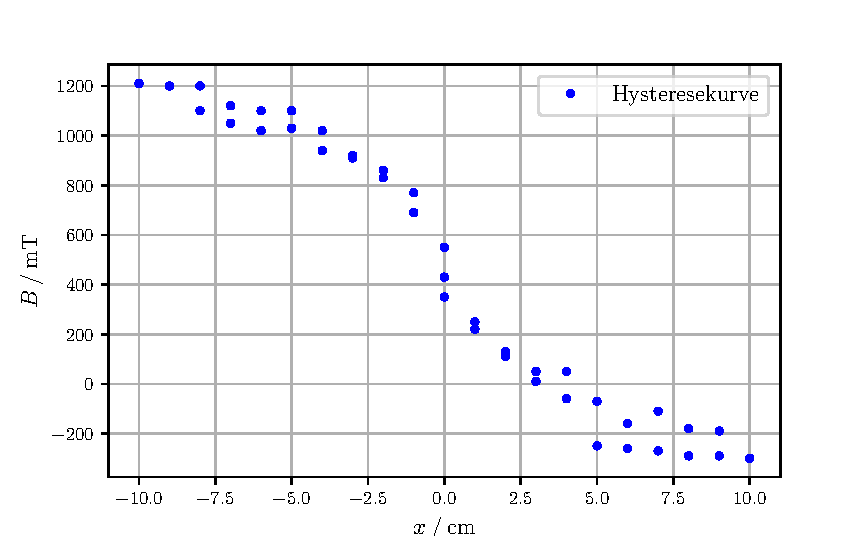
\includegraphics[width=\textwidth]{build/Hysteresekurve.pdf}
  \caption{Messdaten der Ringspule zu einer Hysteresekurve aufgetragen.}\label{fig:hysterese}
\end{figure}


